\chapter{Vorgehen zur Problemlösung}
\section{Einlesen des Grundrisses}
\subsection{Funktionsweise der Bibliothek \textit{kabeja}}
Den Beginn der Verarbeitung markiert hierbei die Grundrissdatei, in welcher sämtliche Werte, welche im weiteren Verlauf des Programmes relevant werden, enthalten sind.
Das Einlesen der Daten eines Grundrisses, wie in Abb. 5, erfolgt mit der Java-Bibliothek „kabeja“. 
Diese ermöglicht es, aus .dxf-Dateien alle DXF-Objekte eines bestimmten Typs zu erhalten und deren Werte in einer Liste zu speichern und später zu verarbeiten \cite{kabeja}.
\begin{code}[DXF File Parser]
public static ArrayList<Line> getAutocadFile(String filePath) throws ParseException {
	ArrayList<Line> vcs = new ArrayList<>();
	Parser parser = ParserBuilder.createDefaultParser();
	parser.parse(filePath, DXFParser.DEFAULT_ENCODING);
	DXFDocument doc = parser.getDocument();
	List lst = doc.getDXFLayer("0").getDXFEntities(DXFConstants.ENTITY_TYPE_LINE);
	for (int index = 0; index < lst.size(); index++) {
		DXFLine dxfline = (DXFLine) lst.get(index);
		Line v = new Line(
		new Vector(round2(dxfline.getStartPoint().getX()), round2(dxfline.getStartPoint().getY())),
		new Vector(round2(dxfline.getEndPoint().getX()), round2(dxfline.getEndPoint().getY())));
		vcs.add(v);
	}
	
	return vcs;
}
\end{code}
In dieser Anwendung wird eine Funktion der Klasse \q{DXFReader} verwendet, welche den Pfad zur .dxf-Datei als Parameter übergeben bekommt. 
Aus dieser Datei werden dann alle DXF-Objekte, die mit dem Typen \icode{DXFLine} übereinstimmen, in einer Liste zurückgegeben. 
Die Koordinaten der Start- und Endpunkte der DXFLines  in dieser Liste werden anschließend in eine Liste von Linien übertragen, welche im weiteren Programmablauf unter anderem für die Umwandlung des Graphen in die DCEL verwendet werden.

\subsection{Funktionsweise der GUI}
Die GUI dient dem Nutzer als Schnittstelle, mit der er die .dxf-Datei auswählt, die er umwandeln möchte.
Die GUI setzt sich hierbei zusammen aus einem \icode{JFrame}, indem ein \icode{JTextField}, ein \icode{FileChooserButton} mit der Aufschrift \q{Choose a file...}, ein \icode{StartButton} mit der Aufschrift \q{Start the conversion} und ein \icode{ShowResultButton} mit der Aufschrift \q{Show the text file} platziert sind.

\begin{Bild}{Ausgangszustand der GUI (Screenshot der Verfasser)}
	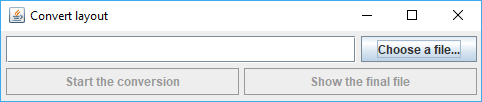
\includegraphics[width = 120mm]{Bilder/GUI_0}
\end{Bild}

Der Nutzer kann im Ausgangszustand über den \icode{FileChooserButton} einen \icode{JFileChooser}-Dialog öffnen, mit dem er die Datei, die er umwandeln möchte, auswählen kann.
Sobald er dann eine Datei ausgewählt hat, wird der Dateipfad zu dieser Datei zusätzlich im \icode{JTextField angezeigt.}
\begin{code} [\icode{JFileChooser} zum Öffnen von Dateien]
JFileChooser fc = new JFileChooser();

int returnVal = fc.showOpenDialog(Main.getGui());
if (returnVal == JFileChooser.APPROVE_OPTION) {
	File file = fc.getSelectedFile();
	Main.getGui().getFilePathField().setText(file.getAbsolutePath());
}
\end{code}

In diesem \icode{JFileChooser} ist außerdem ein \icode{FileFilter} implementiert, der dem Nutzer lediglich .dxf-Dateien anzeigt.

\begin{code} [\icode{FileFilter} innerhalb des \icode{JFileChooser}-Dialogs]
fc.setFileFilter(new FileFilter() {
	public String getDescription() {
		return "DXF Files (*.dxf)";
	}
	public boolean accept(File f) {
		if (f.isDirectory()) {
			return true;
		} else {
			String filename = f.getName().toLowerCase();
			return filename.endsWith(".dxf");
		}
	}
});
\end{code}
\begin{Bild}{Dateiöffnungsdialog (Screenshot der Verfasser)}
	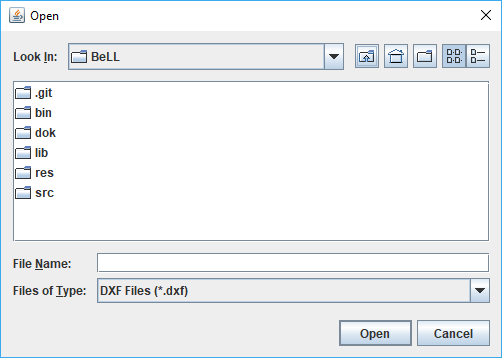
\includegraphics[width = 120mm]{Bilder/GUI_1_FileSelect}
\end{Bild}

Alternativ zum \icode{JFileChooser}-Dialog kann der Nutzer auch direkt in das \icode{JTextField} den Dateipfad eingeben. \\
Nach dem der Nutzer eine existente Datei ausgewählt hat, wird nun der \icode{StartButton} aktiviert und er kann den Konvertierungsprozess starten.

\begin{code} [Aktivierung des \icode{StartButton}]
if (returnVal == JFileChooser.APPROVE_OPTION) {
	File file = fc.getSelectedFile();
	Main.getGui().getFilePathField().setText(file.getAbsolutePath());
	Main.getGui().getStartButton().setEnabled(true);
	Main.startConversion(file.getAbsolutePath());
}
\end{code}
\begin{Bild}{GUI mit aktiviertem \icode{StartButton} (Screenshot der Verfasser)}
	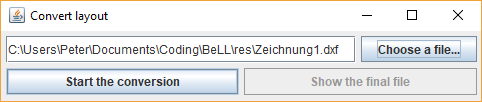
\includegraphics[width = 120mm]{Bilder/GUI_2_InProgress}
\end{Bild}